\documentclass[tikz,border=10pt]{standalone}
\begin{document}
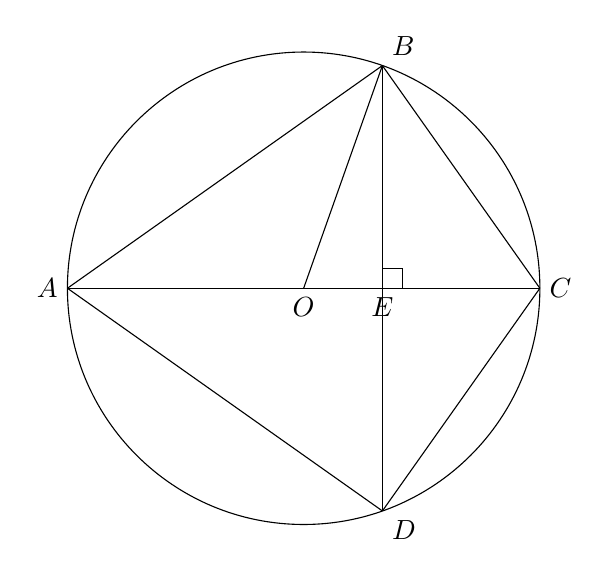
\begin{tikzpicture}
    \coordinate (O) at (0,0);
    \coordinate (A) at (-3,0);
    \coordinate (C) at (3,0);
    \coordinate (E) at (1,0);
    \coordinate (B) at (1, 2.828);
    \coordinate (D) at (1, -2.828);

    \draw (O) circle (3);
    \draw (A) -- (C);
    \draw (B) -- (D);
    \draw (A) -- (B);
    \draw (B) -- (C);
    \draw (C) -- (D);
    \draw (D) -- (A);
    \draw (O) -- (B);

    \draw (1, 0.25) -- (1.25, 0.25) -- (1.25, 0);

    \node[left] at (A) {$A$};
    \node[above right] at (B) {$B$};
    \node[right] at (C) {$C$};
    \node[below right] at (D) {$D$};
    \node[below] at (O) {$O$};
    \node[below] at (E) {$E$};
\end{tikzpicture}
\end{document}
